\documentclass[journal,10pt]{IEEEtran}
\usepackage{amsmath,amssymb}
\usepackage{newtxtext,newtxmath}
\usepackage{booktabs,graphicx,microtype,url}
\usepackage[hidelinks]{hyperref}
\setlength{\emergencystretch}{2em}
\newcommand{\ControlledN}{397}
\newcommand{\ControlledChunks}{34,193}
\newcommand{\ControlledSources}{2,956}
\newcommand{\ControlledPriorAP}{0.6090}
\newcommand{\ControlledQCRAP}{0.8425}
\newcommand{\ControlledAPDelta}{0.2335}
\newcommand{\ControlledAPLower}{0.1850}
\newcommand{\ControlledAPUpper}{0.2841}
\newcommand{\ControlledPriorHit}{0.7683}
\newcommand{\ControlledQCRHit}{0.9446}
\newcommand{\ExternalN}{219}
\newcommand{\ExternalPriorAP}{0.5408}
\newcommand{\ExternalQCRAP}{0.7020}
\newcommand{\ExternalAPDelta}{0.1612}
\newcommand{\ExternalAPLower}{0.0911}
\newcommand{\ExternalAPUpper}{0.2334}
\newcommand{\ExternalPriorHit}{0.6256}
\newcommand{\ExternalQCRHit}{0.7534}
\newcommand{\ExternalIndex}{72.77}
\newcommand{\NaturalVideos}{5,359}
\newcommand{\NaturalEvents}{35,625}
\newcommand{\NaturalCLAPMAP}{0.067576}
\newcommand{\NaturalQCRMAP}{0.052603}
\newcommand{\NaturalCLAPFourMAP}{0.052280}
\newcommand{\NaturalDeltaPoints}{-1.4973}
\newcommand{\NaturalVideoDeltaPoints}{-1.1334}
\newcommand{\NaturalVideoLowerPoints}{-1.4749}
\newcommand{\NaturalVideoUpperPoints}{-0.7804}
\newcommand{\NaturalWorstClassPoints}{-7.1301}
\newcommand{\RouterMAP}{0.096995}
\newcommand{\RouterDeltaPoints}{2.9419}
\newcommand{\RouterRelativeGain}{43.53}
\newcommand{\RouterVideoDeltaPoints}{6.2251}
\newcommand{\RouterVideoLowerPoints}{5.8165}
\newcommand{\RouterVideoUpperPoints}{6.6397}
\newcommand{\CLAPRouterMAP}{0.093921}
\newcommand{\CLAPRouterDeltaPoints}{2.6345}
\newcommand{\IncrementalMAPPoints}{0.3074}
\newcommand{\IncrementalGainShare}{10.45}
\newcommand{\IncrementalVideoPoints}{1.3737}
\newcommand{\IncrementalVideoLowerPoints}{1.1571}
\newcommand{\IncrementalVideoUpperPoints}{1.5895}
\newcommand{\QCRAssignmentPercent}{30.0}
\newcommand{\ActionFormerMAP}{0.116638}
\newcommand{\ActionFormerGapPoints}{1.9643}
\newcommand{\FullPreCapRows}{1,453,945}
\newcommand{\FullFinalRows}{1,044,156}
\newcommand{\FullDiscardedRows}{409,789}
\newcommand{\FullVideosOverCap}{4,401}
\newcommand{\FullMaxPreCap}{356}
\newcommand{\CLAPPreCapRows}{1,662,296}
\newcommand{\CLAPFinalRows}{1,069,264}
\newcommand{\CLAPDiscardedRows}{593,032}
\newcommand{\CLAPVideosOverCap}{5,119}
\newcommand{\CLAPMaxPreCap}{389}
\newcommand{\AnswerSelected}{0.4586}
\newcommand{\AnswerCLAP}{0.4619}
\newcommand{\AnswerStrongest}{0.4780}
\newcommand{\AnswerRandom}{0.4731}
\newcommand{\AnswerOracle}{0.4886}
\newcommand{\AnswerSilence}{0.3877}
\newcommand{\AnswerTextOnly}{0.4033}
\newcommand{\AnswerVsStrongestPoints}{-1.9444}
\newcommand{\AnswerVsStrongestLowerPoints}{-5.2778}
\newcommand{\AnswerVsStrongestUpperPoints}{1.4111}
\newcommand{\UpstreamMaximumDifference}{0.00001873}
\newcommand{\UpstreamReproductionDifference}{5.55e-17}


\title{Where Query-Conditioned Audio Ranking Transfers---and Where It Fails:\\
Controlled Confirmation, Frozen Natural Evaluation, and Cap-Corrected Diagnosis}
\author{Author names and affiliations required before submission}

\begin{document}
\maketitle

\begin{abstract}
Exact-onset mixtures make temporal evidence ranking auditable, but may not
predict localization in natural recordings. We evaluate a five-seed
query-conditioned residual (QCR) ranker that perturbs a pinned CLAP cosine
prior by at most 0.25. On a frozen source-isolated panel, evidence average
precision rises from \ControlledPriorAP\ to \ControlledQCRAP; an external
source-disjoint panel retains a positive \ExternalAPDelta\ gain but misses its
strict absolute-performance gate. We then score all \NaturalVideos\
Perception Test validation videos and \NaturalEvents\ events under a frozen
zero-shot protocol. Multiscale QCR obtains \NaturalQCRMAP\ mAP versus
\NaturalCLAPMAP\ for CLAP, with every temporal-IoU threshold worse and only
two of six gates passing. A disclosed post-outcome, five-fold diagnostic
selects scorer and temporal scale per class, then reapplies one shared
200-segment video cap. It reconstructs all ten capped candidates exactly and
reaches \RouterMAP\ mAP. However, a CLAP-only router reaches
\CLAPRouterMAP; QCR contributes only \IncrementalMAPPoints\ percentage points,
or \IncrementalGainShare\% of the gain over fixed CLAP. The full router remains
below supervised ActionFormer and the learned retrieval fails a held-out
answer bridge. The combined evidence confirms QCR for controlled evidence
ranking, shows that fixed QCR fails zero-shot transfer to natural audio, and identifies
class-dependent temporal scale as the dominant in-domain mechanism. The
cross-fitted result is diagnostic, not fresh confirmation.
\end{abstract}

\begin{IEEEkeywords}
audio event grounding, temporal sound localization, CLAP, transfer
evaluation, cross-fitting, temporal scale, reproducibility
\end{IEEEkeywords}

\section{Introduction}
\IEEEPARstart{T}{ext-conditioned} audio retrieval is frequently studied by
inserting a known sound into a longer background. Exact insertion times make
this design useful: every chunk has a precise overlap label, distractors can
be controlled, and source leakage can be audited. Natural recordings are
harder. Events overlap, vary in duration and loudness, admit ambiguous class
descriptions, and compete under a finite proposal budget. A ranker can
therefore excel at controlled evidence retrieval without transferring to
natural temporal localization.

Contrastive language--audio pretraining (CLAP) provides a transparent
zero-shot similarity between an audio segment and text \cite{clap,laionclap}.
A bounded learned residual may refine this prior, but positive controlled
results leave at least three questions. Does the reordering survive a change
of acoustic construction? Does it survive natural polyphony when temporal
scale and output competition are held fixed? If localization improves, does
that evidence help an audio-language model answer questions?

We address these questions as an evidence ladder rather than forcing one
headline across incompatible stages. The same five frozen QCR checkpoints
first enter a source-isolated exact-onset confirmation and then a
source-disjoint external construction. A one-shot natural transfer protocol
evaluates all 5,359 Perception Test sound-localization validation videos
\cite{perceptiontest}. It freezes prompts, scales, post-processing, caps,
class-macro mean average precision (mAP), a video-paired bootstrap, and six
gates before natural scores exist.

The frozen natural result is negative: multiscale QCR reduces mAP relative to
multiscale CLAP, with all five threshold differences adverse. We retain this
boundary. We then ask a different, explicitly post-outcome question: can a
low-capacity in-domain router diagnose whether scorer or temporal scale is
responsible? Ten CLAP/QCR candidates span 0.5, 1, 2, 4, and pooled scales.
For each of five video-hash folds and ten classes, the candidate is chosen
using only the other four folds. Selected class streams are merged on the held
fold and subjected to one shared 200-segment video cap. A CLAP-only version
isolates scale selection from the residual ranker.

Our contributions are:
\begin{enumerate}
  \item a multi-stage, outcome-faithful evaluation of a bounded
  query-conditioned ranker, including positive controlled evidence and a
  retained negative natural-transfer decision;
  \item a cap-corrected cross-fitting protocol whose candidate pools reproduce
  all original capped outputs exactly before class routing;
  \item a mechanism decomposition showing that class-dependent temporal scale
  accounts for nearly 90\% of the exploratory gain over fixed multiscale
  CLAP, while QCR supplies a smaller positive increment; and
  \item a downstream answer boundary, supervised contextual reference,
  source-linked figures, immutable prediction hashes, protocol invalidations,
  and executable verification.
\end{enumerate}
The post-outcome router is not described as zero-shot or independent
confirmation. Its role is to turn a failed transfer result into a testable
mechanistic diagnosis.

\begin{figure*}[t]
\centering
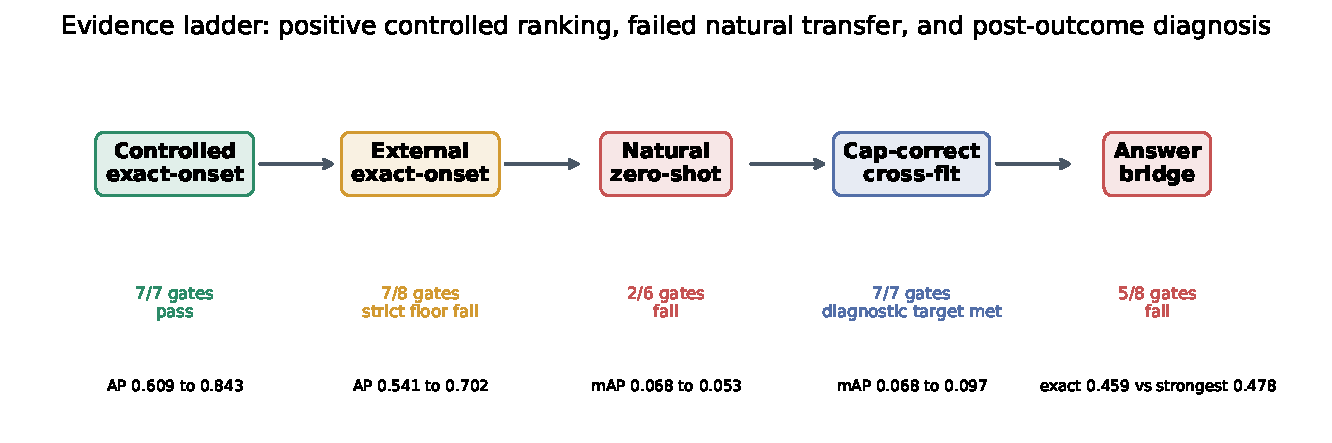
\includegraphics[width=0.98\textwidth]{figures/AEF01.pdf}
\caption{Evidence ladder and immutable decisions. Controlled and natural
endpoints use frozen gate conjunctions. Cross-fitting uses the already exposed
natural validation panel and supports diagnosis only.}
\label{fig:ladder}
\end{figure*}

\section{Related Work}
\subsection{Language--audio representation and grounding}
CLAP aligns audio and text through contrastive pretraining \cite{clap}; the
LAION implementation expands data and studies feature fusion and
keyword-to-caption augmentation \cite{laionclap}. AudioCLIP learns a joint
image--text--audio space \cite{audioclip}, while Wav2CLIP distills audio into
CLIP's visual-language space \cite{wav2clip}. These encoders offer auditable
segment scores but are not trained directly for temporal boundaries.

Text-to-audio grounding links phrases to event times \cite{tag}. Later work
studies cross-modal interaction, suppression of irrelevant regions, and weak
caption supervision \cite{cgi,wstag}. Auto-AEG combines synthetic exact
intervals with pseudo-labeled real audio for scalable open-vocabulary
grounding \cite{autoaeg}. Our study is narrower: queries are renderings of ten
known benchmark classes, and we test whether a ranker developed on controlled
mixtures transfers without natural-label fitting.

\subsection{Sound-event detection and temporal localization}
DESED studies how non-target events, reverberation, label granularity, and
synthetic-versus-recorded data affect event detection \cite{desed}. PSDS
reduces dependence on one operating point and exposes class stability
\cite{psds}. ActionFormer uses multiscale temporal features and boundary
regression for proposal-free localization \cite{actionformer}. Perception Test
adapts temporal localization to diagnostic multimodal video and audio
\cite{perceptiontest}; TIM represents audio/visual time intervals explicitly
\cite{tim}. These results motivate our separation of scale, scorer, class,
and supervision.

\subsection{Cross-fitting and benchmark exposure}
Cross-fitting prevents each held-fold outcome from choosing its own
candidate, but it does not make a reused public validation set untouched.
Our folds estimate a low-capacity in-domain routing rule. Candidate families
were considered after the frozen natural failure, so the result remains
post-outcome exploratory. This distinction is more important than the word
``held-out'': fold isolation controls local selection leakage, whereas fresh
external confirmation requires an unexposed panel.

\section{Query-Conditioned Ranking}
\subsection{CLAP prior and bounded residual}
For audio window $i$ and class query $q$, the pinned unfused CLAP encoder
produces normalized embeddings $\mathbf a_i,\mathbf q\in\mathbb R^{512}$ and
prior
\begin{equation}
p_i=\mathbf a_i^\mathsf{T}\mathbf q.
\end{equation}
Three templates per class are embedded and averaged after normalization. The
QCR ranker projects audio and query embeddings to 64 dimensions; features
include both projections, product, absolute difference, $p_i$, normalized
position, and a sinusoidal position term. Its score is
\begin{equation}
s_i=p_i+0.25\tanh(g_i),
\label{eq:qcr}
\end{equation}
so $|s_i-p_i|\le0.25$ for every proposal. Five checkpoints trained with seeds
0--4 are averaged without seed selection on later panels. Each has 82,759
trainable parameters.

\subsection{Controlled exact-onset task}
A target sound is mixed with backgrounds and distractors. Four-second chunks
at two-second hop receive overlap-derived evidence labels. Evidence AP is the
primary ranking endpoint; exact-onset Hit@1, Recall@4, and top-chunk IoU are
secondary. The source-isolated confirmation contains \ControlledN\ recipes,
\ControlledChunks\ chunks, and \ControlledSources\ unique source files with
zero development-recipe or source overlap. Uncertainty resamples recipes.

The external construction uses UrbanSound8K target clips after excluding
Freesound source IDs present in ESC-50, with fresh LibriSpeech
\texttt{test-other} backgrounds. It contains \ExternalN\ recipes and resamples
original UrbanSound source IDs. Its strict conjunction additionally requires
an absolute performance index $50(\mathrm{AP}+\mathrm{Hit@1})\ge85$.

\section{Natural-Audio Evaluation}
\subsection{Frozen zero-shot protocol}
The natural panel contains all \NaturalVideos\ Perception Test validation
recordings, \NaturalEvents\ annotated events, and ten sound classes. No
Perception Test training label fits QCR. Annotation metadata was inspected to
choose windows $(w,h)$ in seconds:
\[
(0.5,0.25),\ (1,0.5),\ (2,1),\ (4,2).
\]
CLAP and QCR share proposals, prompt ensemble, sigmoid score transform,
Gaussian soft-NMS \cite{softnms}, at most 50 segments per class, and one
200-segment video cap. The four frozen methods are CLAP/QCR at four seconds
and CLAP/QCR with pooled scales.

For class $c$ and temporal-IoU threshold $\tau$, predictions are sorted by
confidence and matched one-to-one to ground-truth intervals. The endpoint is
\begin{equation}
\mathrm{mAP}=\frac1{5}\sum_{\tau\in\{0.1,\ldots,0.5\}}
\frac1{10}\sum_c\mathrm{AP}_{c,\tau}.
\end{equation}
The paired uncertainty summary computes macro AP within each video and
resamples all videos 10,000 times. It is complementary to global class-macro
mAP and can have a different numerical effect size.

Promotion requires all six conditions: positive global difference, positive
video-bootstrap lower endpoint, improvement at at least four thresholds, no
class loss worse than $-0.05$, QCR multiscale at least as good as CLAP at four
seconds, and complete integrity. Prompts, scales, seeds, checkpoints, metric,
and gates cannot change after scoring.

\subsection{Cap-corrected cross-fitted diagnosis}
After the frozen failure, six additional single-scale candidate outputs were
generated, giving CLAP and QCR at 0.5, 1, 2, 4, and pooled scales. The first
exploratory router was invalidated before a report because joining separately
capped class outputs could bypass the shared 200-segment video limit. The
corrected track rebuilds per-class pools before that shared cap and verifies
that reapplying the original cap reconstructs all ten source candidate files
row for row.

A SHA-256 video hash defines five folds. For held fold $f$ and class $c$, the
candidate with highest class AP on the other four folds is selected, with a
stable name tie break. On fold $f$, only that candidate's class-$c$ proposals
are retained. All selected classes are then merged, sorted, and capped once at
200 segments per video. The CLAP-only ablation repeats the procedure with QCR
candidates excluded.

This protocol gives 50 fold--class selections. It uses natural class labels
and an already exposed validation benchmark. Its criteria test internal
coherence---positive global and paired effects, threshold breadth, class
non-harm, cap reconstruction, complete assignment, and integrity---not
zero-shot promotion.

\section{Results}
\subsection{Controlled and external exact-onset evidence}
On the source-isolated confirmation, CLAP evidence AP is
\ControlledPriorAP\ and QCR AP is \ControlledQCRAP, a gain of
\ControlledAPDelta\ with 95\% recipe-bootstrap interval
[\ControlledAPLower,\ControlledAPUpper]. Hit@1 rises from
\ControlledPriorHit\ to \ControlledQCRHit. All five seeds improve and all
seven gates pass.

On the external source-disjoint construction, AP rises from
\ExternalPriorAP\ to \ExternalQCRAP; the \ExternalAPDelta\ gain has 95\%
source-bootstrap interval [\ExternalAPLower,\ExternalAPUpper]. Hit@1 rises
from \ExternalPriorHit\ to \ExternalQCRHit. Seven of eight gates pass. The
declared performance index is \ExternalIndex, below 85, so the strict external
promotion decision remains a failure despite replicated relative gains.

\begin{figure*}[t]
\centering
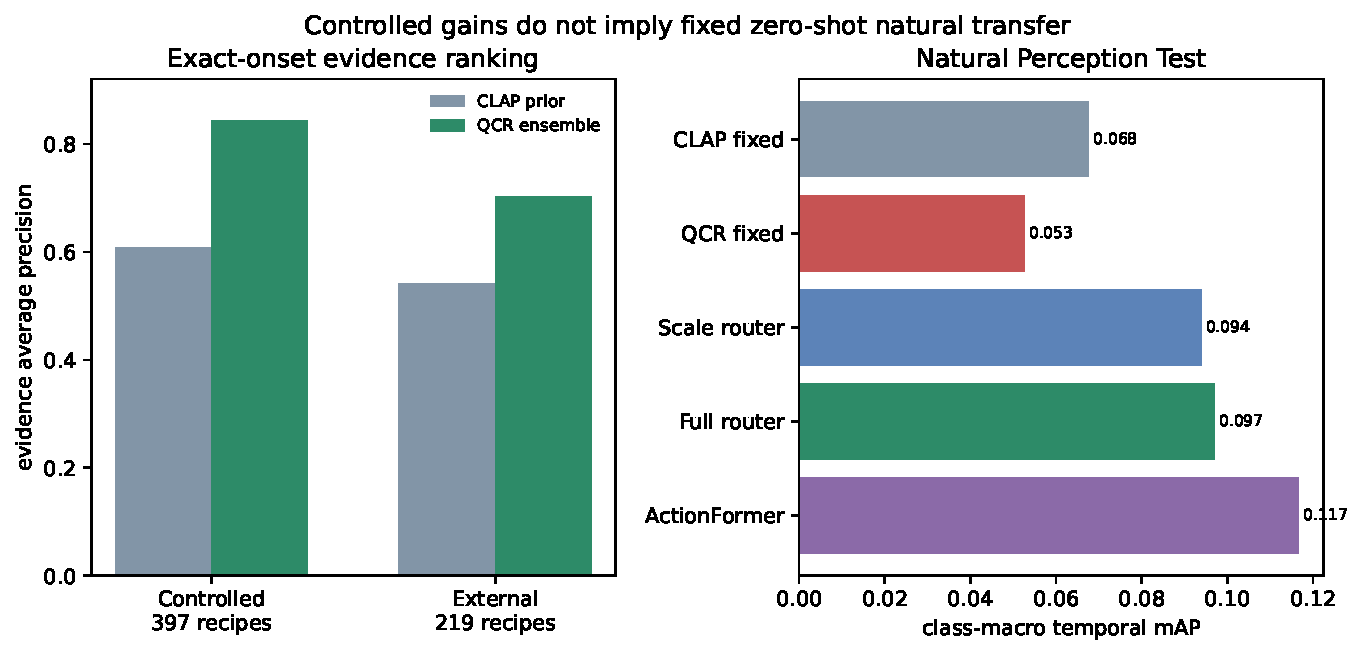
\includegraphics[width=0.98\textwidth]{figures/AEF02.pdf}
\caption{Left: QCR improves exact-onset evidence AP on both controlled
constructions. Right: fixed QCR degrades frozen natural mAP; post-outcome
cross-fitting recovers much of the supervised-context gap. Bars on the right
have different evidence status and are not one leaderboard.}
\label{fig:performance}
\end{figure*}

\begin{table*}[t]
\caption{Evidence-stage ledger. ``Pass'' always refers to that stage's
declared conjunction, not to a universal model claim.}
\label{tab:ledger}
\centering
\footnotesize
\begin{tabular}{lllll}
\toprule
Stage & Evidence status & Panel & Primary contrast & Gates / decision\\
\midrule
Controlled exact-onset & Frozen confirmatory & 397 recipes &
AP $+\ControlledAPDelta$ & 7/7 pass\\
External exact-onset & Frozen external & 219 recipes &
AP $+\ExternalAPDelta$ & 7/8; strict floor fail\\
Natural transfer & Frozen zero-shot & 5,359 videos &
mAP $\NaturalDeltaPoints$ pp & 2/6 fail\\
Cap-correct router & Post-outcome cross-fit & same validation &
mAP $+\RouterDeltaPoints$ pp & 7/7 diagnostic criteria\\
Answer bridge & Held-out downstream & 411 examples &
exact $\AnswerSelected$ vs.\ $\AnswerStrongest$ & 5/8 fail\\
\bottomrule
\end{tabular}
\end{table*}

\subsection{Frozen natural transfer failure}
Multiscale CLAP obtains \NaturalCLAPMAP\ mAP; multiscale QCR obtains
\NaturalQCRMAP. The frozen QCR-minus-CLAP difference is
\NaturalDeltaPoints\ percentage points. All five temporal-IoU differences are
negative. The paired-video mean change is \NaturalVideoDeltaPoints\ points,
with interval [\NaturalVideoLowerPoints,\NaturalVideoUpperPoints] and zero of
10,000 replicates above zero. The worst class change is
\NaturalWorstClassPoints\ points. Only the scale-floor and integrity gates
pass.

\begin{figure}[t]
\centering
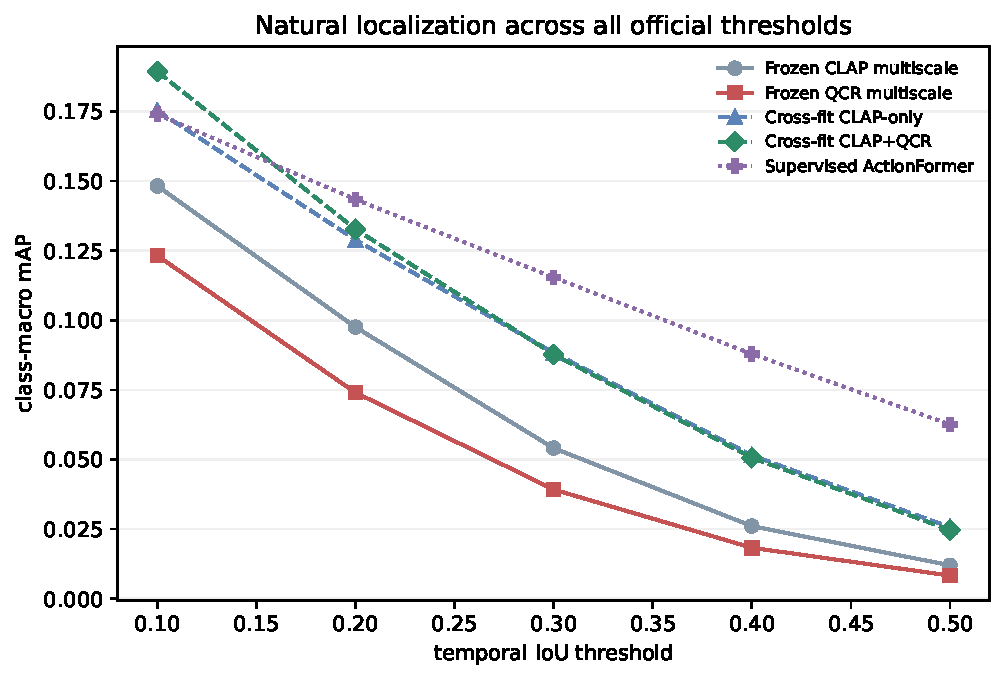
\includegraphics[width=\columnwidth]{figures/AEF03.pdf}
\caption{Natural class-macro mAP at every official tIoU threshold. Fixed QCR
is below fixed CLAP throughout. Cross-fitted curves are post-outcome; the
ActionFormer curve is supervised context.}
\label{fig:thresholds}
\end{figure}

The official supervised audio-only ActionFormer checkpoint obtains
\ActionFormerMAP\ mAP under the same recomputed metric. It uses Perception Test
training labels and official features, so it is context rather than a
zero-shot gate.

\subsection{What cap-corrected cross-fitting diagnoses}
The full cap-corrected router obtains \RouterMAP\ mAP versus
\NaturalCLAPMAP\ for fixed multiscale CLAP, a gain of
\RouterDeltaPoints\ points (\RouterRelativeGain\% relative). Every threshold
and class difference is positive. The paired-video macro-AP effect is
\RouterVideoDeltaPoints\ points with interval
[\RouterVideoLowerPoints,\RouterVideoUpperPoints]. All seven diagnostic
criteria pass.

The CLAP-only router already obtains \CLAPRouterMAP, a gain of
\CLAPRouterDeltaPoints\ points over fixed CLAP. Adding QCR raises global mAP
by only \IncrementalMAPPoints\ points, \IncrementalGainShare\% of the total
gain. Its post-hoc paired-video increment is \IncrementalVideoPoints\ points
with interval [\IncrementalVideoLowerPoints,\IncrementalVideoUpperPoints].
Thus QCR has a positive in-domain increment, but class-dependent scale choice
is the dominant mechanism.

\begin{table}[t]
\caption{Natural localization status and decomposition.}
\label{tab:natural}
\centering
\footnotesize
\begin{tabular}{lrl}
\toprule
Method & mAP & Evidence role\\
\midrule
Fixed CLAP multiscale & \NaturalCLAPMAP & frozen zero-shot comparator\\
Fixed QCR multiscale & \NaturalQCRMAP & frozen zero-shot primary\\
Cross-fit CLAP-only & \CLAPRouterMAP & post-outcome scale diagnosis\\
Cross-fit CLAP+QCR & \RouterMAP & post-outcome full diagnosis\\
ActionFormer audio & \ActionFormerMAP & supervised context\\
\bottomrule
\end{tabular}
\end{table}

QCR is selected for \QCRAssignmentPercent\% of the 50 fold--class
assignments. Nine of ten classes choose the same candidate in all folds.
Speech and animal sound prefer QCR at four seconds; dropping prefers QCR at
one second. Clapping selects half-second CLAP, fluid selects two-second CLAP,
and the remaining classes choose one-, two-, or four-second CLAP. This
stability explains why a pooled-scale score is not optimal under cross-class
proposal competition.

\begin{figure*}[t]
\centering
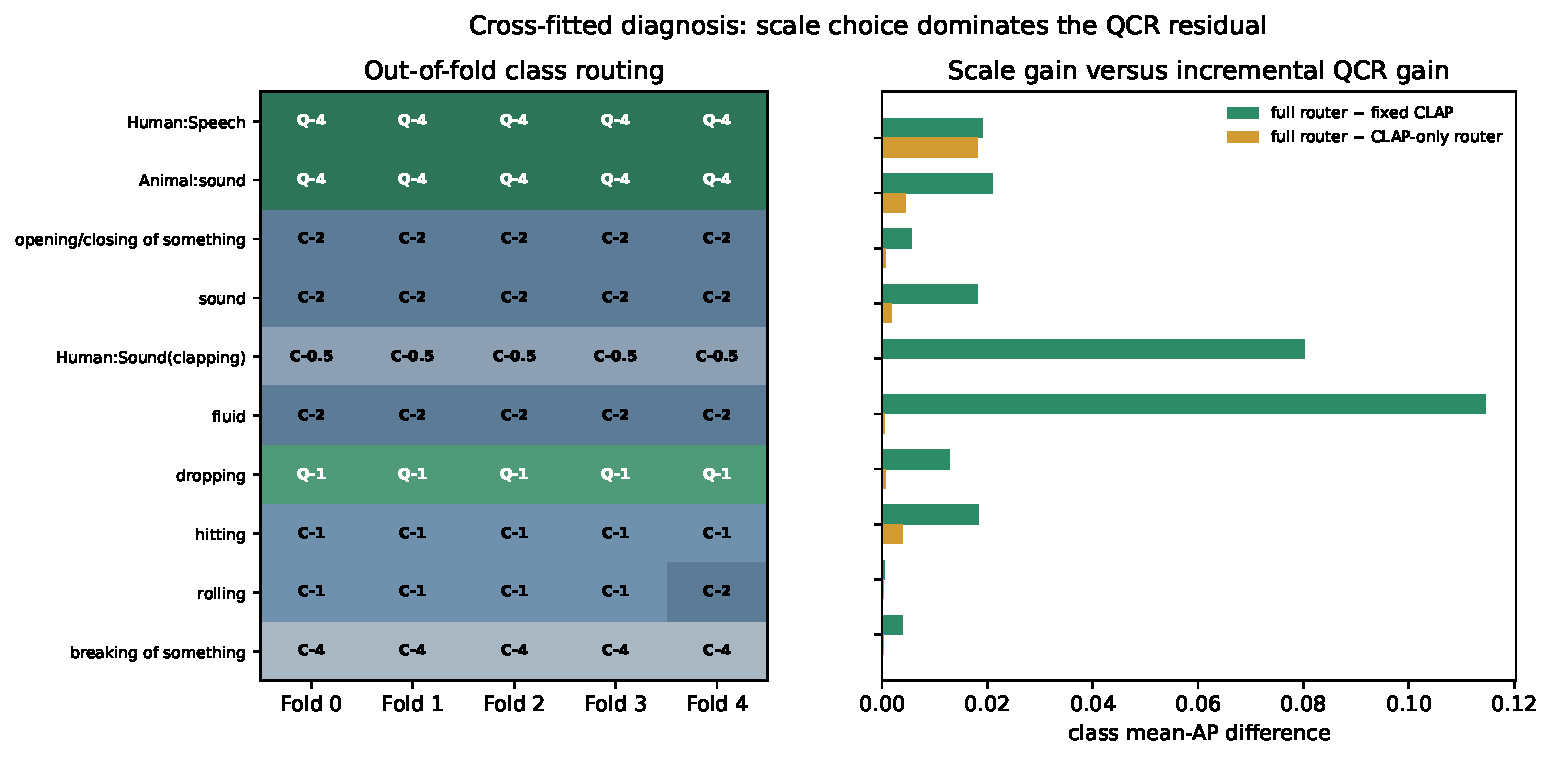
\includegraphics[width=0.98\textwidth]{figures/AEF04.pdf}
\caption{Left: selected candidate for every held fold and class
(\(C\)=CLAP, \(Q\)=QCR, number=window seconds). Nine classes are unanimous.
Right: the full router's gain over fixed CLAP is large for clapping and fluid;
the incremental QCR gain beyond the CLAP-only router is smaller but positive
for every class.}
\label{fig:routing}
\end{figure*}

The full route merges \FullPreCapRows\ proposals, discards
\FullDiscardedRows\ under the shared limit, and writes \FullFinalRows\
predictions; \FullVideosOverCap\ videos exceed 200 proposals before capping.
The CLAP-only route is audited identically. All ten candidate reconstructions
are exact, no output video exceeds 200 segments, and no metric is nonfinite.
The full router remains \ActionFormerGapPoints\ points below supervised
ActionFormer.

\subsection{Downstream answer boundary}
On 411 held-out answer examples from 25 sources and two audio-language
decoders, learned QCR retrieval obtains two-backbone source-macro exact
accuracy \AnswerSelected. CLAP retrieval obtains \AnswerCLAP, deterministic
random retrieval \AnswerRandom, the strongest eligible prefix-matched
baseline \AnswerStrongest, and oracle spans \AnswerOracle. The learned method
passes five of eight gates and does not improve answer accuracy. This result
is compatible with the localization analysis: overlap AP does not ensure that
a fixed-duration span contains the evidence a decoder needs.

\section{Discussion}
\subsection{A transfer boundary, not a contradictory result}
Controlled and natural tasks differ in both data and relevance structure. In
exact-onset mixtures, one inserted target defines positive chunks and
distractors are engineered. In natural audio, several valid events can
overlap, class durations differ, and all class proposals compete under a
shared cap. QCR's bounded residual can learn a useful controlled ordering and
still harm the fixed natural ordering. The frozen negative result is therefore
a direct measurement of construct transfer, not a failed implementation.

\subsection{Why temporal scale dominates}
Short impulses such as clapping benefit from half-second windows, while
speech and broad object sounds prefer longer context. Pooling every scale
does not merely add recall: it changes proposal density and soft-NMS/cap
competition. Per-class selection recovers 2.63 mAP points with CLAP alone.
QCR adds 0.31 points globally and a positive video-paired increment, mainly
where longer speech/animal windows or one-second dropping windows are useful.
This decomposition suggests that future zero-shot work should model
query-conditioned temporal resolution before adding a more expressive
residual scorer.

\subsection{What remains to be confirmed}
Cross-fitting prevents a held video's own outcomes from selecting its
candidate, and 9/10 class choices are fold-stable. It does not undo candidate
design after benchmark exposure, class-label supervision, or reuse of the
public validation split. A fresh natural dataset with an independently frozen
router is required to test the diagnosis. Until then, \RouterMAP\ is an
in-domain exploratory estimate rather than a new zero-shot headline.

\section{Threats to Validity}
\paragraph{Construct validity.}
Class-macro temporal AP rewards annotated overlap. It does not measure
explanation, causal reasoning, source separation, or answer sufficiency.
Queries are three templates for ten known classes, not unconstrained
open-vocabulary language.

\paragraph{Internal validity.}
The candidate pools reproduce all ten capped source files exactly. A first
router was invalidated because its class join could violate the shared cap;
no router report from that attempt is used. The corrected analyzer's only
post-freeze code amendment replaces a quadratic cap assertion with an
equivalent linear count. Both records are retained.

\paragraph{Metric validity.}
The frozen implementation differs slightly from the pinned upstream
ActionFormer evaluator in stable tie ordering and floating-point tIoU
association. Reproducing both upstream semantics matches upstream class AP
within \UpstreamReproductionDifference; the maximum frozen-versus-upstream
mAP difference is \UpstreamMaximumDifference, and every metric-dependent
frozen gate remains unchanged.

\paragraph{External and statistical validity.}
Perception Test contains ten everyday sound classes and short recordings.
Results need not transfer to music, bioacoustics, meetings, long recordings,
new languages, or strongly polyphonic scenes. Video bootstraps summarize this
finite panel; classwise diagnostic criteria are not multiplicity-adjusted
hypothesis tests.

\section{Reproducibility, Rights, and Compute}
The release includes protocols, freeze and amendment locks, QCR checkpoint
hashes, exact candidate-cap reconstruction receipts, full and CLAP-only
router predictions, natural predictions, aggregate reports, source data,
tests, and independent verifiers. Raw benchmark audio, CLAP weights, official
ActionFormer features/checkpoint, UrbanSound8K, ESC-50, and LibriSpeech remain
with their providers. Exact URLs, revisions, checksums, and acquisition
instructions are retained; non-commercial source restrictions are disclosed.

All natural embeddings use the same pinned CLAP encoder and verified
precompute backend. The largest frozen QCR residual is below the analytic
0.25 bound. Cross-fit candidate pools are excluded from the compact
submission archive because they are regenerable derived intermediates; their
row counts and SHA-256 values remain in the receipt.

\section{Conclusion}
A bounded residual ranker can be genuinely effective for controlled
exact-onset evidence retrieval yet fail fixed zero-shot localization in
natural audio. Retaining that failure and enforcing the shared output cap
reveals the main mechanism: class-dependent temporal scale, not the QCR
residual, supplies most of the in-domain cross-fitted gain. QCR adds a smaller
positive increment, but the diagnostic router remains post-outcome and below
supervised ActionFormer; it also does not improve held-out answers. The result
is a sharper, reproducible boundary on where query-conditioned ranking
transfers and what must be confirmed next.

\section*{Author Declarations}
Names, affiliations, ORCIDs, corresponding contact, CRediT roles, funding,
competing interests, data-license review, and any required AI-assistance
disclosure must be supplied and approved by the accountable authors before
submission. No new human-subject data were collected; the study analyzes
public benchmark releases under their stated terms.

\begin{thebibliography}{99}
\bibitem{clap} B. Elizalde, S. Deshmukh, M. Al Ismail, and H. Wang,
``CLAP: Learning audio concepts from natural language supervision,''
in \emph{Proc. IEEE ICASSP}, pp. 1--5, 2023.
\bibitem{laionclap} Y. Wu, K. Chen, T. Zhang, Y. Hui,
T. Berg-Kirkpatrick, and S. Dubnov, ``Large-scale contrastive
language--audio pretraining with feature fusion and keyword-to-caption
augmentation,'' in \emph{Proc. IEEE ICASSP}, pp. 1--5, 2023.
\bibitem{audioclip} A. Guzhov, F. Raue, J. Hees, and A. Dengel,
``AudioCLIP: Extending CLIP to image, text and audio,''
in \emph{Proc. IEEE ICASSP}, pp. 976--980, 2022.
\bibitem{wav2clip} H.-H. Wu, P. Seetharaman, K. Kumar, and J. P. Bello,
``Wav2CLIP: Learning robust audio representations from CLIP,''
in \emph{Proc. IEEE ICASSP}, pp. 4563--4567, 2022.
\bibitem{tag} X. Xu, H. Dinkel, M. Wu, and K. Yu, ``Text-to-audio grounding:
Building correspondence between captions and sound events,''
in \emph{Proc. IEEE ICASSP}, pp. 606--610, 2021.
\bibitem{cgi} H. Tang, Y. Wang, J. Zhu, S. Zhang, M. Xu, Q. Zheng, and
Y. Hu, ``Listen as you wish: Audio-based event detection via text-to-audio
grounding in smart cities,'' arXiv:2106.14136, 2021.
\bibitem{wstag} X. Xu, Z. Ma, M. Wu, and K. Yu, ``Towards weakly supervised
text-to-audio grounding,'' arXiv:2401.02584, 2024.
\bibitem{autoaeg} Z. Zhang, X. Cheng, W. Yan, T. Zhang, D. Fu, B. Zhang,
Y. He, and T. Jin, ``Auto-AEG: Scalable data construction for open-vocabulary
audio event grounding,'' arXiv:2607.04383, 2026.
\bibitem{desed} N. Turpault, R. Serizel, S. Wisdom, H. Erdogan,
J. Hershey, E. Fonseca, P. Seetharaman, and J. Salamon, ``Sound event
detection and separation: A benchmark on DESED synthetic soundscapes,''
in \emph{Proc. IEEE ICASSP}, pp. 840--844, 2021.
\bibitem{psds} C. Bilen, G. Ferroni, F. Tuveri, J. Azcarreta, and
S. Krstulovi\'c, ``A framework for the robust evaluation of sound event
detection,'' in \emph{Proc. IEEE ICASSP}, pp. 61--65, 2020.
\bibitem{actionformer} C. Zhang, J. Wu, and Y. Li, ``ActionFormer:
Localizing moments of actions with Transformers,'' in \emph{Proc. ECCV},
pp. 492--510, 2022.
\bibitem{perceptiontest} V. P\u{a}tr\u{a}ucean \emph{et al.},
``Perception Test: A diagnostic benchmark for multimodal video models,''
in \emph{Advances in Neural Information Processing Systems}, vol. 36, 2023.
\bibitem{tim} J. Chalk, J. Huh, E. Kazakos, A. Zisserman, and D. Damen,
``TIM: A time interval machine for audio-visual action recognition,''
in \emph{Proc. IEEE/CVF CVPR}, pp. 18153--18163, 2024.
\bibitem{softnms} N. Bodla, B. Singh, R. Chellappa, and L. S. Davis,
``Soft-NMS---Improving object detection with one line of code,'' in
\emph{Proc. IEEE ICCV}, pp. 5561--5569, 2017.
\end{thebibliography}

\end{document}
